\section{Experiments}

We validate the algorithmic implications of our theory on image and text classification tasks.
First, we show that our proposed metric is able to predict positive or negative transfer using only STL performances.
Second, we show that MTL can improve data efficiency ratio.
Finally, we show that performing covariance alignment is more significant when the source task data size is large compared to the target task.

\subsection{Experimental Setup}

{\bf Datasets and models.} We describe the datasets and models we use in the experiments.

{\it Sentiment Analysis:} This dataset includes six tasks: movie review sentiment (MR), sentence subjectivity (SUBJ), customer reviews polarity (CR), question type (TREC), opinion polarity (MPQA), and the Stanford sentiment treebank (SST) tasks.

{For each task, the goal is to categorize sentiment opinions expressed in the text.
We use an embedding layer (with GloVe embeddings\footnote{http://nlp.stanford.edu/data/wordvecs/glove.6B.zip}) followed by an LSTM layer proposed by~\cite{lei2018simple}.
}
%multi-layer perceptron (MLP), LSTM, CNN on all tasks
%We use this task to verify our theoretical results on model capacity and task covariance in real world.

{\it ChestX-ray14:} This dataset contains 112,120 frontal-view X-ray images and each image has up to 14 diseases.
This is a 14-task multi-label image classification problem.
%We treat each label as one task a binary classification problem and formulate it as a 14-task multi-task learning problem.
%This dataset is curated where the labels
%We use the CheXNet model from~\cite{chexnet}, which is a 121-layer convolutional neural network on all tasks.

For all models, we share the main module across all tasks and assign a separate regression or classification layer on top of the shared module for each tasks.

\subsection{Improving training efficiency in MTL}

\subsection{Validating the Algorithmic Implications}

\textbf{A metric to determine positive or negative transfer.}
We validate the metric proposed in Section \ref{sec_similarity} for predicting positive or negative transfer based on STL results.
Table \ref{tab:mtl_better_than_stl} shows that using a threshold of $0.1$, we can predict $75.6\%$ among 150 task pairs for the sentiment analysis tasks with $38.8\%$ recall.
Similar for 91 image classification task pairs.
Note: For text classification tasks, the source task training data size ranges from 500 to 1,500 and target task training data size is 1000; For ChestX-ray14, the training data size is 10,000.

\begin{table}
\begin{minipage}[t]{.58\textwidth}
	\centering
  \begin{tabular}{c c c c c}
	\toprule
		\multirow{2}{*}{{\bf Threshold}}  & \multicolumn{2}{c}{{\bf Text
		classification}} & \multicolumn{2}{c}{{\bf ChestX-ray14}} \\
		& Precision &  Recall & Precision &  Recall \\
		\cmidrule(lr){1-1} \cmidrule(lr){2-3} \cmidrule(lr){4-5}
		0.0 & 0.596 & 1.000 & 0.593 & 1.000 \\
		0.1 & 0.756 & 0.388 & 0.738 & 0.462 \\
		0.2 & 0.919 & 0.065 & 0.875 & 0.044 \\	
		% 0.3 & 1.000 & 0.004 &     - &     - \\
	\bottomrule
	\end{tabular}
	\vspace{0.1in}
	\captionof{table}{Ablation study on when should use MTL via different source/target task accuracy.}
	\label{tab:mtl_better_than_stl}
\end{minipage}
\quad
% \vspace{}
\begin{minipage}[t]{.40\textwidth}
	\centering
	\begin{tabular}{c c c}
		\toprule
		\multirow{2}{*}{{\bf Models}} & \multicolumn{2}{c}{\begin{minipage}{1.1in}\begin{center}
		MR, SST, SUBJ, CR, MPQA, TREC\end{center}\end{minipage}} \\
		\cmidrule(lr){2-3}
		& {\bf Standard} & {\bf Alignment} \\
		\midrule
		{\bf MLP}  & > 100\% & 39\% \\
		{\bf LSTM} & 36\% & 36\% \\
		\bottomrule
		\end{tabular}
	\vspace{0.1in}
	\captionof{table}{Taskonomy experiment.}
	\label{tab:taskonomy}
\end{minipage}
\end{table}

% \begin{table}
% \begin{center}
%   \begin{tabular}{c c c c c}
%   \toprule
%     \multirow{2}{*}{{\bf Threshold}}  & \multicolumn{2}{c}{{\bf Text classification}} & \multicolumn{2}{c}{{\bf ChestX-ray14}} \\
%     & Precision &  Recall & Precision &  Recall \\
%     \cmidrule(lr){1-1} \cmidrule(lr){2-3} \cmidrule(lr){4-5}
%     0.0 & 0.596 & 1.000 & 0.593 & 1.000 \\
%     0.1 & 0.756 & 0.388 & 0.738 & 0.462 \\
%     0.2 & 0.919 & 0.065 & 0.875 & 0.044 \\	
%     0.3 & 1.000 & 0.004 &     - &     - \\
%   \bottomrule
%   \end{tabular}
% \end{center}
% \caption{Ablation study on when should use MTL via different source/target task accuracy.}
% \label{tab:mtl_better_than_stl}
% \end{table}

\textbf{MTL improves labeled data efficiency.}
We measure the data efficiency ratio on the sentiment analysis tasks.
We find that by performing multi-task learning, only $39\%$ of the labeled data is needed to achieve comparable performance to single-task learning over all six tasks.
If TREC is not included, we see that only $25\%$ of the labeled data is needed.


\textbf{Covariance alignment.}
We validate that the performance of aligning task covariances depends on the size of source task data.
In Figure \ref{fig_covariate}, we observe that the benefit from aligning task covariances becomes more significant as we increase the size of the source task dataset.

\begin{figure}[!ht]
	\centering
	\begin{subfigure}[b]{0.33\textwidth}
		\centering
		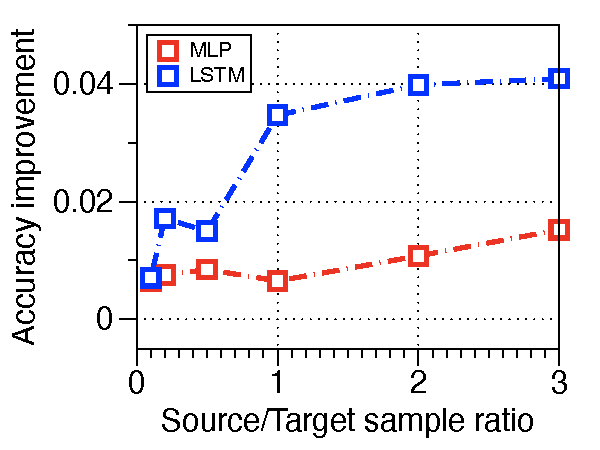
\includegraphics[width=0.975\textwidth]{figures/ratio_alignment_norm_diff_all.pdf}
		\caption{Averaged}
	\end{subfigure}\hfill
	\begin{subfigure}[b]{0.33\textwidth}
		\centering
		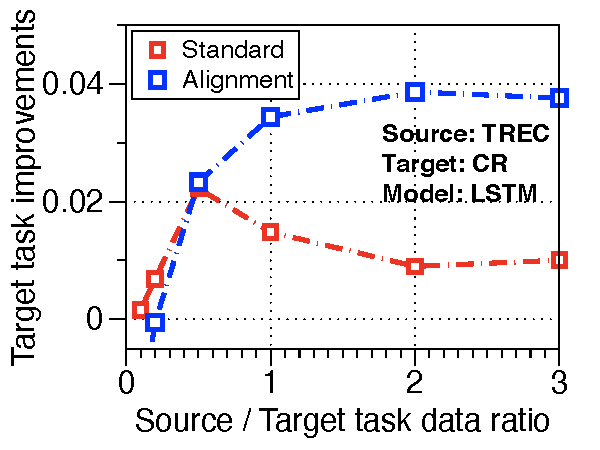
\includegraphics[width=0.975\textwidth]{figures/ratio_alignment_norm_trec_cr_lstm.pdf}
		\caption{Task pair TREC and CR}
	\end{subfigure}\hfill
		\begin{subfigure}[b]{0.33\textwidth}
		\centering
		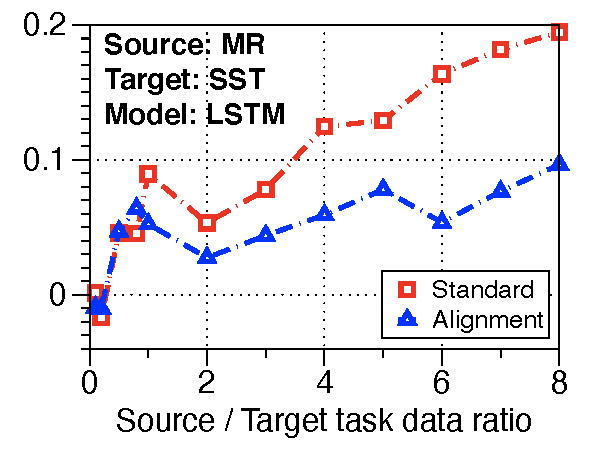
\includegraphics[width=0.975\textwidth]{figures/ratio_alignment_mr_sst_lstm.pdf}
		\caption{Task pair MR and SST}
	\end{subfigure}
	\caption{The performance of aligning task covariances depends on data size. As the ratio between source task data size and target task data size increases, the performance improvement from aligning task covariances increases.}
	\label{fig_covariate}
\end{figure}


%\subsection{Validating Theoretical Implications}


%\textbf{Contributing causes of negative transfer.}

%\textbf{Implications for positive learning.}



%\textit{Transferring from a high accuracy to low accuracy.}%%%%%%%%



% \begin{table}
% 	\begin{center}
% 		\begin{tabular}{c c c c c}
% 		\toprule
% 		\multirow{2}{*}{{\bf Models}} & \multicolumn{2}{c}{\begin{minipage}{1.1in}\begin{center}
% 		MR, SST, SUBJ, CR, MPQA, TREC\end{center}\end{minipage}} & \multicolumn{2}{c}{\begin{minipage}{1.1in}\begin{center}MR, SST, SUBJ, CR, MPQA\end{center}\end{minipage}} \\
% 		\cmidrule(lr){2-3} \cmidrule(lr){4-5}
% 		& {\bf Standard} & {\bf Alignment} & {\bf Standard} & {\bf Alignment} \\
% 		\midrule
% 		{\bf MLP}  & > 100\% & 39\% & 25\% & 25\% \\
% 		{\bf LSTM} & 36\% & 36\% & 28\% & 25\% \\
% 		% {\bf CNN}  & 76\% & - & 32\% & -\\
% 		\bottomrule
% 		\end{tabular}
% 	\end{center}
% 	\caption{Taskonomy experiment.}
% 	\label{tab:taskonomy}
% 	\end{table}


%\begin{figure}
%	\centering
%	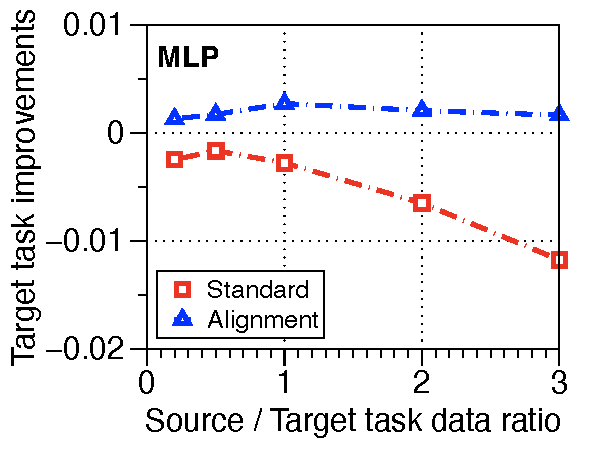
\includegraphics[width=0.5\textwidth]{figures/ratio_alignment_mlp.pdf}
%	\caption{Covariate shift experiment.}
%\end{figure}
